%----------------------------------------------------------------------------
\chapter{A hálózaton kipróbált algoritmusok}
%----------------------------------------------------------------------------
Ebben a fejezetben bemutatom az általam megírt algoritmusokat, amelyeket ezen hálózaton teszteltem, és egyben összehasonlítom egy méretben kisebb, fiktív gráfon is alkalmazva. Az algoritmusok programozási nyelve a C++, amely eltér az eddig használt nyelvtől. Ugyanakkor ezt a nyelvet választottam, mert ezeket a programokat később más diáktársak is felhasználhatják a gráfelméleti algoritmika elsajátításakor. Így viszonyítani tudom a sok fontos információt és tanácsot az egyetemnek, ha ez csak egy kis töredéke annak, amit én tanulhattam az elmúlt évek során.

Következzenek az általam megvalósított algoritmusok, amelyeket  a hálózat szociáis jellegű vizsgálatára készítettem :
\section{A pletyka terjedése}
\begin{figure}[!h]
	\centering
	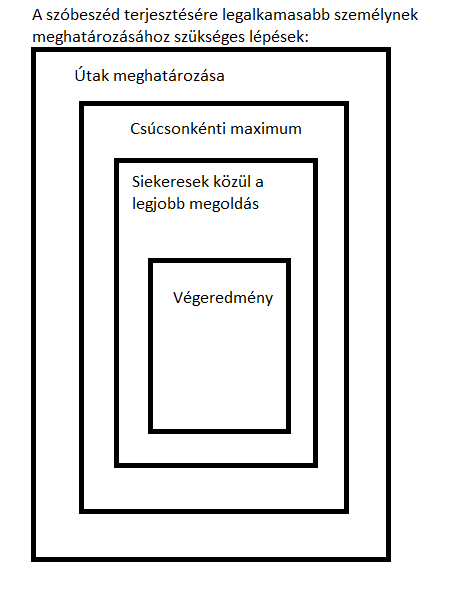
\includegraphics[scale=0.45]{images/elsoprogram}
	\caption{Szoftver lépései}
\end{figure}
Az első algoritmus a két pont közötti út meghatározására használt algoritmus továbbképzése, amelynek köszönhetően a szociológiai elemként tartott pletyka (szóbeszéd) milyen gyorsan tud terjedni, akár e-mailek által, egy nagyobb hálózaton keresztül.
Ezen program felépítése több lépésből áll, amelynek első lépése egy mélységi bejárás egy irányított gráfon, majd a második lépésben minden csúcsra meghatározzuk az utat, vagyis hogy az üzenet egyik személytől a másik személyig hány emberen keresztül jut el.

Ugyanakkor az utolsó lépésben meghatározom, hogy a hálózatban ki lenne a legjobb központ, ki által terjed a legjobban a pletyka, valamint melyik személy nem tudja eljuttatni mindenhová a szóbeszédet.

Látványos áttekintésként az alábbi gráfot hoznám fel, amely segítségével könnyebb megérteni a fent említett információkat.


\begin{figure}[!h]
	\centering
	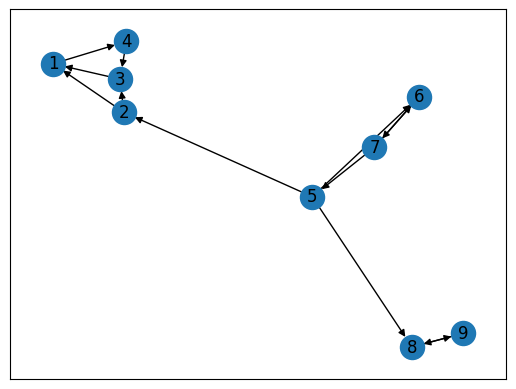
\includegraphics[scale=0.6]{images/kisgraf}
	\caption{Gráf a szóbeszédhez}
\end{figure}

Az ábrán látható egy 9 csúcspontból álló irányított gráf, amelyet azért készítettem, hogy érthetőbb legyen az algoritmus magyarázata.

Az első lépés a mélységi bejárás által meghatározni az utakat. A képen is látható, hogy az 1 pontból csak a 4 és 3 pontig jutunk el, tehát itt az üzenet csak 2 személyhez jut el. Hasonlóképpen nem jutunk messze a 2., 3. és 4. pontokkal sem. Az 5. pont már minden más csúcshoz el tudja küldeni az üzenetet. A leghosszabb út, amit megtesz az üzenet, a 4-es elemhez való információ közlést alkotja. Ehhez át kell mennie 2 ponton (2. és 1. csúcsokon), ami pontosan 3 él hosszú. Ezt a leghosszabb utat eltároljuk, valamint azt is, hogy összesen hány él mentén kellett bejárnia az utakat. Az utóbbi adat azért szükséges, ha van még egy hasonló elem, akkor ez dönti el, ki van a középpontban. De térjünk át egy másik olyan pontra, amely be tudja járni az egész gráfot, ez a pont a 7-es. A kiválasztott pont annyiban tér el az 5-östől, hogy a leghosszabb útja 4 él hosszú. Ezért a döntés az 5-ösre esik, így ő lesz a hálózat központja. Tehát az ő által küldött üzenetek érnek el mindenhová, és mindezt a legoptimálisabb idő alatt tudja elérni.

A kis példa után áttérnék az általam felhasznált 50 fős adattömegre, amelynek vizualizációját már bemutattam. Ugyanakkor bemutatom a programot, amelyet használtam az előző gráfnál is. Mint tudjuk, a gráfok nagysága és éleinek száma nagyban eltér, ezért összehasonlítottam a futási időket. A hamarosan megjelenített program a kis gráfra, amely 9 csúcsot és 12 élet tartalmaz, 0,0094 másodperc alatt végezte el a középpont megkeresését és annak pontos meghatározását, míg az 50 ezres és még szűrés nélküli, 80 000 fölötti üzeneteket tároló fájl használata során 0,0467 másodpercet volt képes elérni.

\newpage
Következzen is a C++ szoftver bemutatása és annak magyarázata:


\begin{figure}[!h]
	\centering
	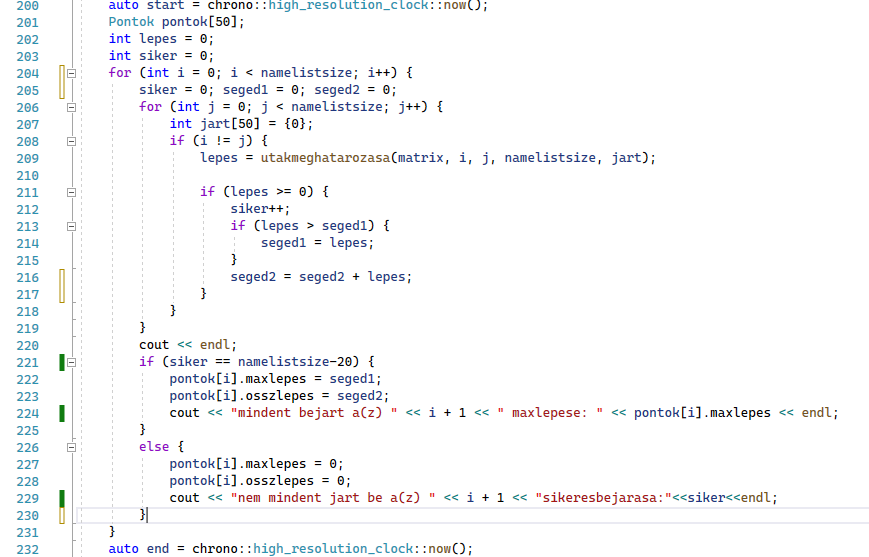
\includegraphics[scale=0.7]{images/utaskod}
	\caption{két pont közötti út távolság meghatározása}
\end{figure}

Az első képen látható egy függvény, amely, ahogy említésre került, az első lépésre íródott. Tehát meghatározza két pont között, hogy van-e út, és ha van, akkor az hány él hosszúsággal rendelkezik. Ennek a függvénynek összesen 5 paramétere van. Sorrendben egy két dimenziós tömb, tehát egy mátrix, majd az 'st' változó, amely egy valós számot tartalmaz, és a kezdő pontot határozza meg, vagyis hogy honnan kell indulni az út meghatározásához. A harmadik paraméter a végső pont indexét határozza meg, majd ezek után következik a méret, amely segíti a mátrix bejárását, és végül egy tömb, amelyben rögzítem, hogy az adott ponton már jártam-e. Ezzel a tömbbel ki tudom küszöbölni a gráfban keletkező körök létrejöttekor felmerülő végtelen ciklust.
A 't' és 'mint' változók a jelenlegi út hosszát tárolják, majd ezek közül a minimumot választják.

Kezdésként ellenőrzöm, hogy ha van kapcsolat az indulási pont és az úticél között, akkor megkapom, hogy az út hossza 1, és visszatérek vele. Ha nincs kapcsolat, akkor beállítom, hogy jártam a kezdő pontban, majd áttérek azokra az esetekre, amikor minden olyan útvonalat ellenőrzök, amely a kezdőpontból indul és valamerre halad. Ha nincs ilyen útvonal, akkor visszatérek -1 értékkel, amivel jelezem, hogy nincs út a két pont között. Ha van olyan eset, hogy a program tovább tud lépni a kezdőpontból, vagyis van kimenő éle a pontnak, akkor ebben az esetben hívom meg újra a függvényt, amikor már eljutottam a pozícióhoz. Ezzel a meghívással hozom létre a rekurziót.

A minimális út kiválasztása az alábbi módon történik: Ha már van értéke a 'mint' változónak, és nagyobb az eddig meghatározott útnál ('t'-nél), akkor megváltoztatom annak értékét. Ugyanakkor, ha a 'mint' változó továbbra is -1, és kapok egy helyes útvonalat, vagyis változott a 't' értéke, akkor visszaadom újra a 't' értékét. Abban az esetben, ha a 't' soha nem változik, akkor a 'mint' értéke változatlan marad, és a program -1 értéket térít vissza. De ha a 'mint' értéke változott, akkor az adott értékhez hozzáadok 1-et, és ezt a függvény visszatéríti, mivel ebben az esetben a következő ponttól volt számolva a távolság.

\newpage
\begin{figure}[h]
	\centering
	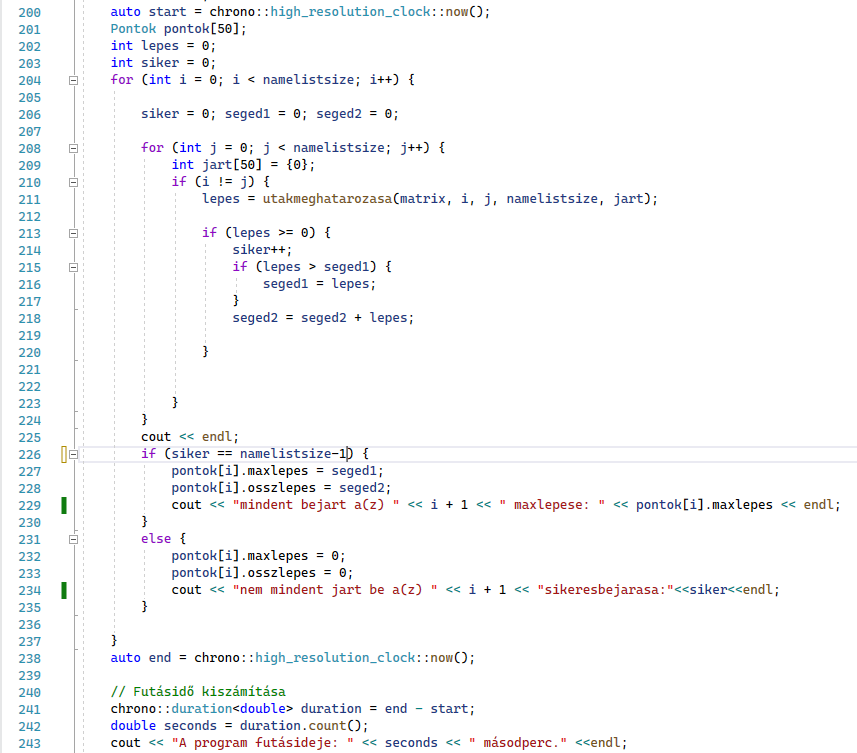
\includegraphics[scale=0.6]{images/kozeppont}
	\caption{Utak meghatározása és középső pont kiderítése}
\end{figure}

A fenti képen látható az algoritmus főbb része, amely során beolvasott adatokat feldolgozza a program, meghatározza minden csúcs által bejárt utak összegét, valamint ezek közül a legnagyobb út hosszát. Kivételt képeznek azok a csúcsok, amelyek nem tudnak üzenetet küldeni mindenkinek. A program minden érték esetén kiírja, hogy az adott személy elért-e mindenkit, és ha igen, akkor mekkora a maximális út, amit egy személy elérése során megtett.

A fenti képen látható, hogy az algoritmus futási ideje mérve van (200., 232. sor), és az eredményben is megjelenik ennek kiíratása.

\begin{figure}[h]
	\centering
	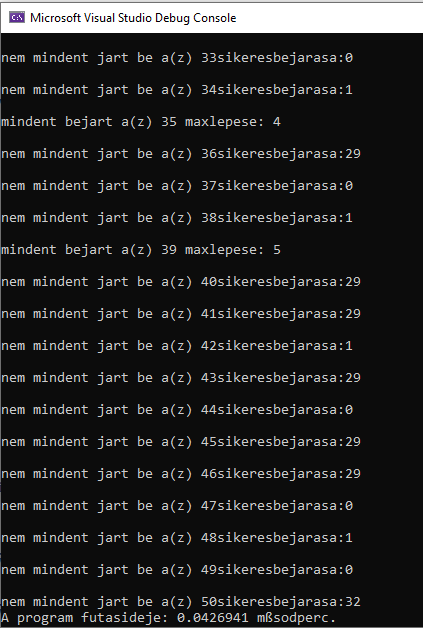
\includegraphics[scale=0.4]{images/utaseredmeny}
	\caption{Eredmény kiíratása}
\end{figure}

\section{A csomósodási együttható kiszámítása}

Mi az a csomósodási együttható? A csomósodási együttható egy érték, amely a gráfokban a csúcsokhoz kapcsolódik, és az adott pont szomszédok közötti kapcsolatot vizsgálja. Ez az érték egy aránynak tekinthető, amely maximum 1 lehet. Az arány két összetevőből áll: a szomszédok között lehetséges kapcsolatok száma és a létrejött kapcsolatok száma. A csomósodási együttható segítségével meg lehet határozni, hogy mennyi valószínűsége van annak, hogy egy pont barátai egymással is kapcsolatban állnak. Minél kevesebb szomszéddal rendelkezik egy csúcs, annál nagyobb az esélye annak, hogy közelíti az 1-hez tartó értéket.

Mi a csomósodási együttható célja? A csomósodási együttható mérése segít megérteni, hogyan változik a hálózat dinamikája az új élek hozzáadásával. Ha új élek kerülnek a gráfba, ez az érték növekedhet, és megfelelő mennyiségű él hozzáadásával általában eléri az 1-es értéket. Ha minden pont csomósodási együtthatója 1, akkor bármely pont kiválasztása esetén a szomszédok egy teljes gráfot alkotnak.

Összefoglalva, a csomósodási együttható az hálózat dinamikájának figyelésére szolgáló érték, amely rámutat a pontok közötti kapcsolatok kialakulására.

A használt hálózatot szép és látványos eredmények érdekében átalakítottam az irányított gráfból egy irányítatlan hálózattá. Ennek az átalakításnak az alapja az volt, hogy ha az x pont küld egy e-mailt az y pontnak, akkor az y pont ismeri az x pontot. Az alábbi ábrán bemutatom a szoftver lényeges részeit:
\begin{itemize}
    \item Kezdeném az elsődleges függvénnyel, amelyet a második lépésben felhasználok. Ez a függvény segít meghatározni az adott pont szomszédai között kialakult kapcsolatok, azaz élek számát. A függvény egy számot ad vissza, és a paraméterei között szerepel egy mátrix, amely tárolja a pontok közötti éleket. Emellett megkap egy tömböt is, amelyben szerepel a szomszédok listája, valamint a szomszédsági lista hossza is felhasználható harmadik paraméterként.

A függvény a mátrix bejárása során meghatározza, hány él található a szomszédok között, és ezt az értéket az 'eredmény' változóban tárolja. Ezután az eredményt visszatéríti.
    \begin{figure}[h]
    \centering
    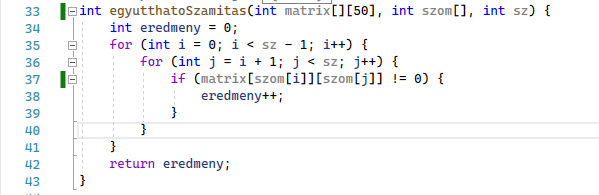
\includegraphics[scale=1 ]{images/egyutthatoszamitas}
    \caption{Együttható kiszámításához használt függvény}
    \end{figure}
    
    \item A második kódrészletben látható az összes csomósodási együttható kiszámítása és tárolása.

Ebben a részben a program használója beolvashat egy számot, amely a csomópontok között szerepel, és válaszként megkapja a félévente lekérdezett csomósodási együttható értékét. A program az adott személyek közötti kapcsolatokat rendezett elküldési időpont szerint növekvő sorrendbe, így jobban megfigyelhetővé válik a hálózat dinamikája.

    
    \begin{figure}[h]
    \centering
    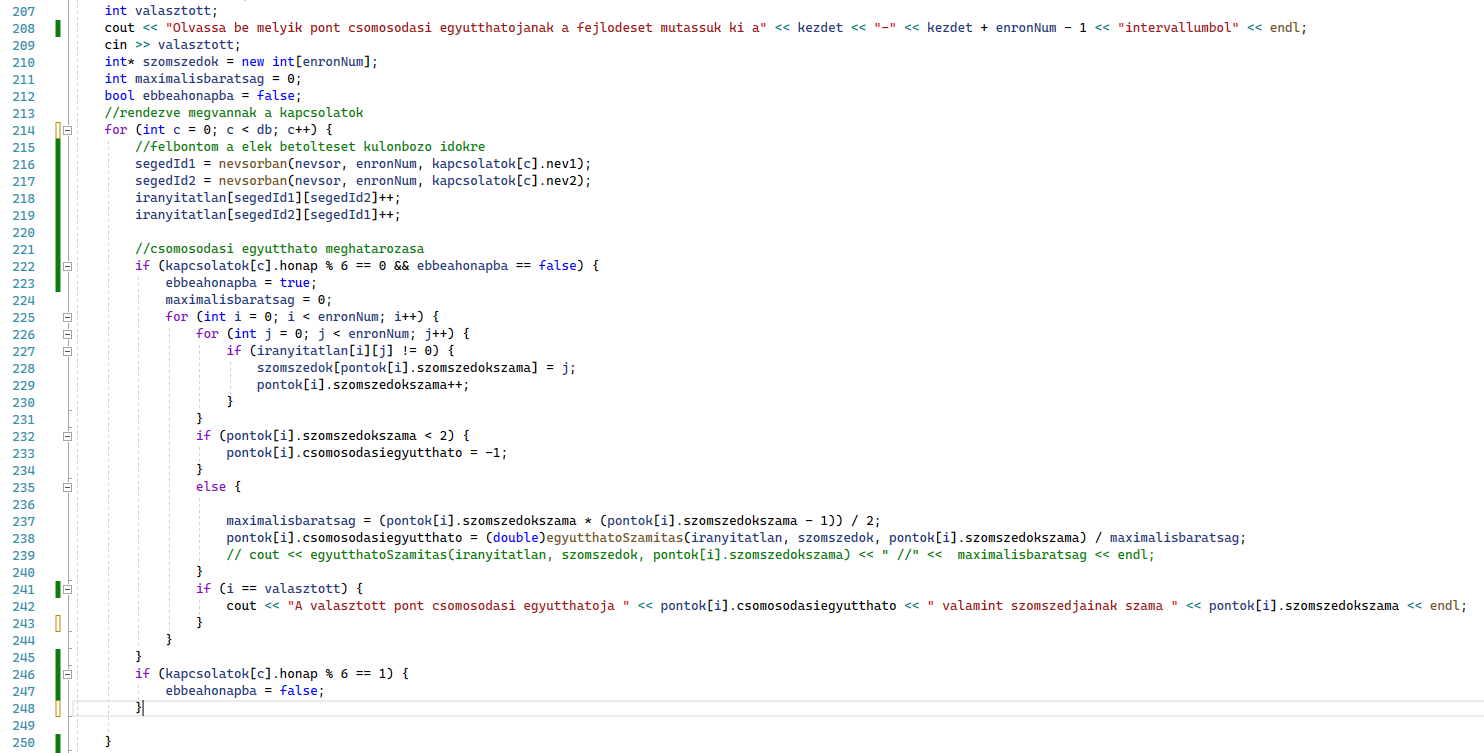
\includegraphics[scale=0.5 ]{images/egyutthato}
    \caption{Csomósodási együttható meghatározása időközönként}
    \label{fig:enter-label}
    \end{figure}

    A fenti kódrészletben a szűrésen és rendezésen áteső kapcsolatokat bejárva feltöltődik az irányítatlan gráf. Ez a feltöltés megszakad minden 6 hónapban, amikor a csomósodási pontok kiszámításai történnek. Ahhoz, hogy egy hónapban csak egyszer mérjünk, bevezettem az 'ebbenahonapba' nevű bool típusú változót, amely akkor vált igazra, ha már történt mérés az adott hónapban. Minden első és hetedik hónapban visszaállítom a változót hamisra (false). Az újbóli bejutás a mérésbe csak a 6-tal osztható hónapokban lehetséges.

Hogyan zajlik egy mérés? Egy mérés során megvizsgálom, hogy minden pontnak hány szomszédja van, és ezt beállítom az adott pontnak. Ezután két lehetőséget zárok ki: ha egy pontnak 1 vagy 0 szomszédja van. Ha egy pontnak 1 szomszédja van, akkor annak nem lehet más kapcsolata, és ha 0 szomszédja van, akkor sem lehet kiszámolni a pont csomósodási együtthatóját. Ha a szomszédok száma meghaladja az 1-et, akkor már kiszámítható az együttható.

    Az együttható meghatározásának képlete :
    \[
		Együttható=\leg\frac{Szomszédok Közötti Kapcsolatok Száma}{SzomszédokSzáma*(SzomszédokSzáma-1)/2}.
    \]

    Ugyanakkor beszéljek néhány használt függvényről és változóról. A program kezdetén bekérek egy 1 és 50 közötti számot, amely meghatározza a gráf méretét. Ez a változó neve 'enronNum' (210. sor). A szomszédok dinamikus tömböt használok, amelyben tárolom a pontok jelenlegi szomszédjait a kapcsolatok meghatározásához. A maximális barátság változó a fenti képletben látható osztó értékét fogja tárolni az eredmény számításához. A 'segedId1' és 'segedId2' változók a nevsorban függvény visszatérési értékét tárolják, amely egy int típusú elem lesz, mert a függvény visszaadja a nevsorban szereplő email indexét. Majd a meghatározott indexekből létrehozott éleket bevezetem az irányítatlan gráfot tartalmazó mátrixba. Ezzel már bemutattam az összes változót, amely a képen látható. Emellett említeném még a Kapcsolat típusú változót, amelyből egy tömb van létrehozva a kapcsolatok tárolására. Ennek az elemnek van két karakterláncot tartalmazó név1 és név2 változója, valamint egy három számból álló értéke a dátum kezelhetősége miatt.
    \begin{figure}[h]
        \centering
        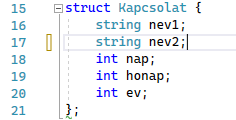
\includegraphics[scale=1]{images/kapcsolat}
        \caption{Kapcsolat struktúra}
        
    \end{figure}
    \item Utolsó megjegyzésként szeretném megmutatni egy algoritmus eredményét, amely egy 50 elemű gráf esetén, 3923 éllel rendelkezve az 5 pont csomósodási együtthatóját jeleníti meg 6 hónapos lépésekkel. Emellett a program végén meghatározom, melyik csúcs, vagyis személy rendelkezik a legnagyobb együtthatóval, feltéve, hogy a pontok számának legalább az ötödével van kapcsolatban. Végül, az utolsó eredményként meghatározom a legtöbb szomszéddal rendelkező személyt a gráfból.
    \begin{figure}[h]
        \centering
        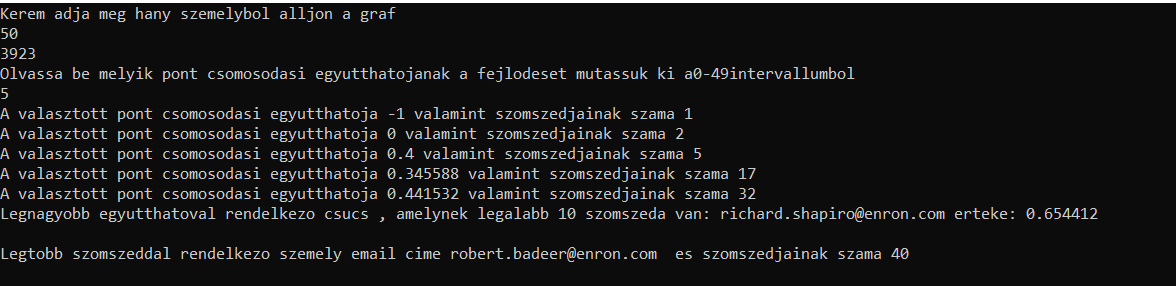
\includegraphics[scale=0.6]{images/eredmeny2}
        \caption{Változás az együtthatókban}
        
    \end{figure}
\end{itemize}

\section{Az hálózat kapcsolatainak vizsgálata}

Ebben a részben a kapcsolatok fontosságával foglalkoztam, és azt vizsgáltam, hogy egy kapcsolat, üzenetváltás mennyire fontos a hálózatban. Azért fontos egy ilyen nagy hálózatban, mert akár egyetlen egy kapcsolat, kötődés két egyén között is jelentős hatással lehet a hálózatra. Ha töröljük vagy megszüntetjük az adott kapcsolatot, az egész hálózat több részre szakadhat. Ezt a szétesést a gráfoknál úgy érhetjük el, hogy töröljük az egyik élt, amely egy hídat alkotott két komponens között.
\newpage

Az alábbi gráfon is látható , hogy a 3-1 él hídat képez a 2 háromszöget kirajzoló ponthalmazok között.
\begin{figure}[h]
    \centering
    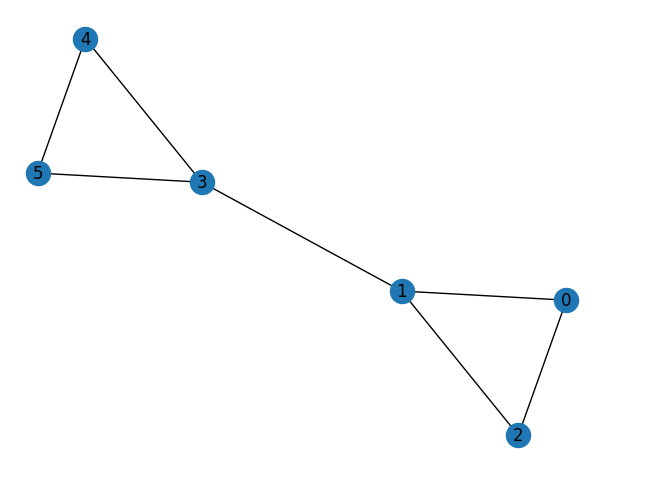
\includegraphics[scale=0.5]{images/hid}
    \caption{Gráf a híd magyarázatához}
    \label{fig:enter-label}
\end{figure}

A második ábrán megfigyelhető különbség segít megérteni a lokális híd kialakulásának könnyed magyarázatát. Amikor a 1-3 él törlésre kerül, még mindig képesek kommunikálni egymással az üzenetek, de a bejárás során megfigyeljük, hogy a két pont közötti távolság megnövekszik. Ha ez a növekedés meghaladja a 2 egységet, akkor a törölt élet lokális hídnak nevezzük.


\begin{figure}[h]
    \centering
    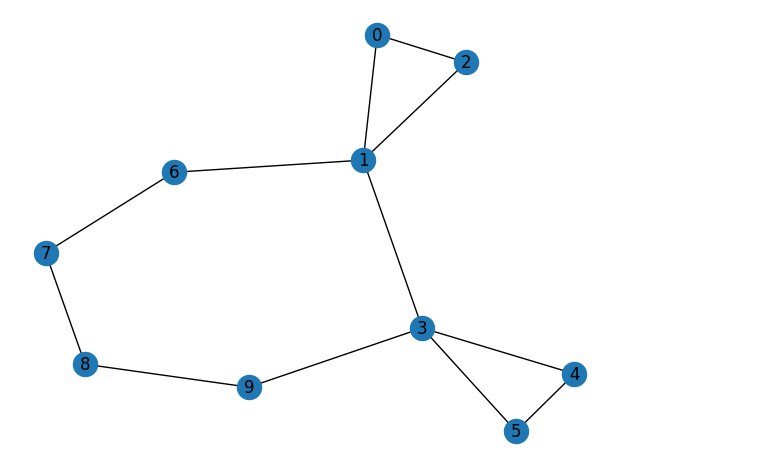
\includegraphics[scale=0.5]{images/lokalishid}
    \caption{Gráf a lokálishíd magyarázatához}
    \label{fig:enter-label}
\end{figure}
 
És mire is jó, ha tudjuk, hogy egy él híd vagy sem? A hídek lehetővé teszik két vagy több komponens összekapcsolását, így összefüggő gráfokkal tudunk dolgozni. Ugyanakkor a hídek nélkül is lehet az hálózat összefüggő, de ekkor lehetnek benne lokális hídek. Ha egy összefüggő gráfban nincs híd, és nincsenek lokális hídek sem, akkor nagy valószínűséggel teljes gráfról beszélünk.

Ezeket a jelenségeket vizsgáltam az általam használt adatokon, és a következő kis kódrészletekben bemutatom a kutatás lépéseit.

Az algoritmus legfontosabb eleme egy mélységi bejárás, amelyet a legrövidebb út meghatározásához is használtam a dolgozathoz szükséges szoftverek megírásában. A bejárás segítségével el tudom dönteni, hogy két pont között, ha törlöm az élt, akkor marad-e út a két csúcs között. Ennek egyik alapvető része az, hogy az irányított gráfot átalakítottam irányítatlan gráffá, mivel egy irányított gráfban nagyon nehéz két pont között több utat keresni, mivel kevesen válaszolnak az üzenetekre. Ezért szemléletesebbnek találtam, ha irányítatlan gráfon tesztelem a csúcsokat.

\begin{figure}[h]
    \centering
    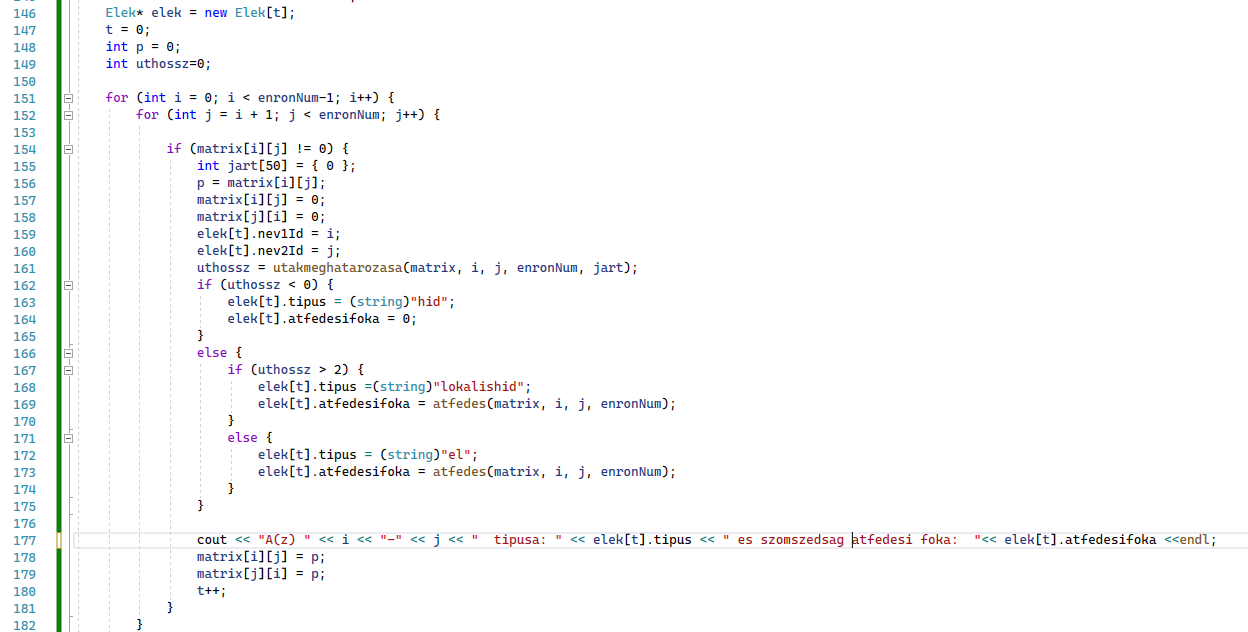
\includegraphics[scale=0.5]{images/hidprogram}
    \caption{Híd meghatározása}
    \label{fig:enter-label}
\end{figure}
 A fenti program részben megfigyelhető egy egymásba ágyazott 'for' ciklus, amely az éleket keresi meg és velük végzi el a műveleteket. Először megvizsgálja, hogy egy adott él létezik-e két pont között. Ha igen, akkor átírja annak értékét egy változóba, majd törli az élt (az értékét 0-ra állítja). A törölt éllel rendelkező mátrixszal meghívja a két pont közötti útvonalat kereső függvényt, amely egy számot ad vissza. Ha a visszatérített érték kisebb mint 0, akkor nincs kapcsolat a két pont között, tehát a törölt él híd volt. Ha az útvonal hossza meghaladja a 2 egységet, akkor a törölt élnek lokális híd jellegzetességet adunk. Ha az előző két eset nem teljesül, akkor az él átlagosnak tekintett jellegű marad.

Az élek tulajdonságainak tárolására egy Élek struktúrát hoztam létre, amely tartalmazza a küldő és címzett információkat, a szomszédsági átfedést, az él jellegét tároló lehetőséget, valamint a később említett köztességi fokszámát.


\begin{figure}[h]
    \centering
    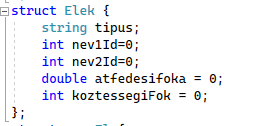
\includegraphics[scale=1.1]{images/elek}
    \caption{Él struktúra}
    \label{fig:enter-label}
\end{figure}

Ahogy az előző gondolatban is említésre került a következő tulajdonság amely az élekhez tartozik  a szomszédsági átfedés.Ezen változó kiszámítása hasonlóan a pontok csomósodási együtthatójához, egy olyan arány határoz meg, amely az él két végpontjának a közös szomszédjait és az mindkét pont összes szomszédjának számát használja fel.A kódrészlet magyarázata előtt kis ábrával pontosítanám ezen átfedetségi változó értékének fogalmát, melyben a pontok színbeli eltérésével szemléletesebb a különség és könnyen észrevehető , hogy miből is áll ez az érték.
\newpage

\begin{figure}[h]
    \centering
    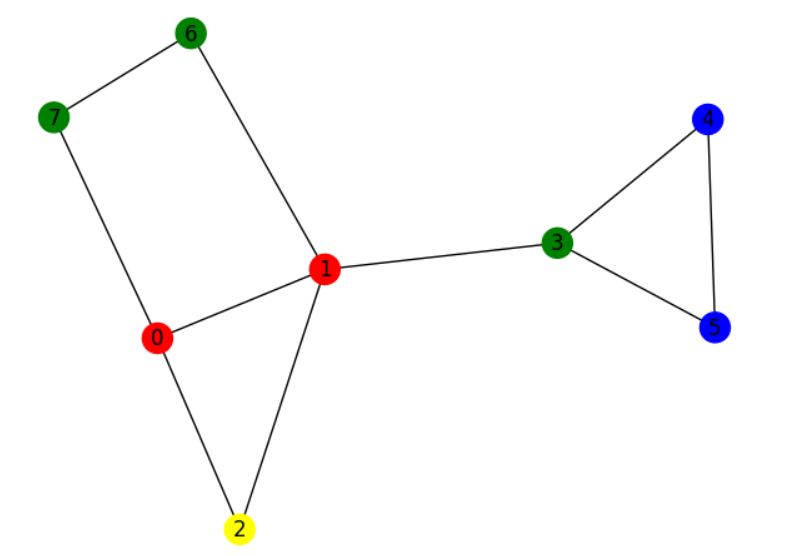
\includegraphics[scale=0.4]{images/atfedesi}
    \caption{Átfedéshez használt példa gráf}
    \label{fig:enter-label}
\end{figure}

Ahogy az előző részben is említésre került, az élekhez tartozik a szomszédsági átfedés tulajdonság. Ennek a változónak a kiszámítása hasonló módon történik, mint a pontok csomósodási együtthatójának meghatározása. Ez az arány meghatározza az él két végpontjának közös szomszédjainak számát és az összes szomszédjának számát mindkét pontnál. Az ábrával kísérve pontosítom ezen átfedési változó értékének fogalmát, ahol a pontok különböző színekkel vannak jelölve, hogy szemléletesebb legyen a különbség és könnyen észrevehető legyen, hogy ez az érték miből áll.

\begin{figure}[h]
    \centering
    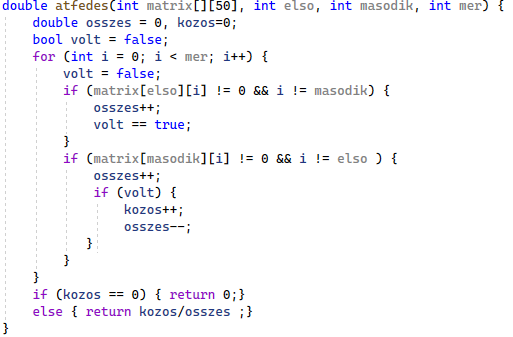
\includegraphics[scale=0.6]{images/atfedesikod}
    \caption{Átfedés számításához használt függvény}
    \label{fig:enter-label}
\end{figure}


A függvény paraméterlistája egy mátrixot tartalmaz, amelyben az élek vannak tárolva. A második paraméter az él indulási pontját határozza meg, és a függvény megvizsgálja ennek a pontnak a szomszédjait. Ezután a harmadik paraméterrel ismét ugyanezt a műveletet végzi el. Az utolsó paraméter meghatározza, hogy hány csúcsból áll a gráf. Ha ez a szám kevesebb, mint 50, akkor az "i" változónak nem kell 50-ig iterálnia a "for" ciklusban.

A közös szomszédok kiválasztása egy segéd "bool" típusú változóval van megoldva. Ez a változó csak akkor vesz fel igaz értéket, ha az "i"-dik csúcsnak van közös szomszédja az első elemmel. Ha a második elem is kapcsolatban van az "i"-dik elemmel, akkor azt közös szomszédnak számolom, és visszavonom az összes szomszéd számának növelését. A bejárás után, ha a közös változó értéke 0 maradt, akkor a függvény 0-t ad vissza, különben pedig egy 0 és 1 közötti értéket.
